\documentclass[]{book}
\usepackage{lmodern}
\usepackage{amssymb,amsmath}
\usepackage{ifxetex,ifluatex}
\usepackage{fixltx2e} % provides \textsubscript
\ifnum 0\ifxetex 1\fi\ifluatex 1\fi=0 % if pdftex
  \usepackage[T1]{fontenc}
  \usepackage[utf8]{inputenc}
\else % if luatex or xelatex
  \ifxetex
    \usepackage{mathspec}
  \else
    \usepackage{fontspec}
  \fi
  \defaultfontfeatures{Ligatures=TeX,Scale=MatchLowercase}
\fi
% use upquote if available, for straight quotes in verbatim environments
\IfFileExists{upquote.sty}{\usepackage{upquote}}{}
% use microtype if available
\IfFileExists{microtype.sty}{%
\usepackage{microtype}
\UseMicrotypeSet[protrusion]{basicmath} % disable protrusion for tt fonts
}{}
\usepackage{hyperref}
\hypersetup{unicode=true,
            pdftitle={Eesti inimarengu aruanne 2019},
            pdfauthor={Eesti Koostöö Kogu},
            pdfborder={0 0 0},
            breaklinks=true}
\urlstyle{same}  % don't use monospace font for urls
\usepackage[style=authoryear]{biblatex}
\ExecuteBibliographyOptions{refsegment=chapter}
\addbibresource{bibliography/bib\_chapter23.bib}
\addbibresource{bibliography/bib\_chapterXY.bib}
\usepackage{longtable,booktabs}
\usepackage{graphicx,grffile}
\makeatletter
\def\maxwidth{\ifdim\Gin@nat@width>\linewidth\linewidth\else\Gin@nat@width\fi}
\def\maxheight{\ifdim\Gin@nat@height>\textheight\textheight\else\Gin@nat@height\fi}
\makeatother
% Scale images if necessary, so that they will not overflow the page
% margins by default, and it is still possible to overwrite the defaults
% using explicit options in \includegraphics[width, height, ...]{}
\setkeys{Gin}{width=\maxwidth,height=\maxheight,keepaspectratio}
\IfFileExists{parskip.sty}{%
\usepackage{parskip}
}{% else
\setlength{\parindent}{0pt}
\setlength{\parskip}{6pt plus 2pt minus 1pt}
}
\setlength{\emergencystretch}{3em}  % prevent overfull lines
\providecommand{\tightlist}{%
  \setlength{\itemsep}{0pt}\setlength{\parskip}{0pt}}
\setcounter{secnumdepth}{5}
% Redefines (sub)paragraphs to behave more like sections
\ifx\paragraph\undefined\else
\let\oldparagraph\paragraph
\renewcommand{\paragraph}[1]{\oldparagraph{#1}\mbox{}}
\fi
\ifx\subparagraph\undefined\else
\let\oldsubparagraph\subparagraph
\renewcommand{\subparagraph}[1]{\oldsubparagraph{#1}\mbox{}}
\fi

%%% Use protect on footnotes to avoid problems with footnotes in titles
\let\rmarkdownfootnote\footnote%
\def\footnote{\protect\rmarkdownfootnote}

%%% Change title format to be more compact
\usepackage{titling}

% Create subtitle command for use in maketitle
\providecommand{\subtitle}[1]{
  \posttitle{
    \begin{center}\large#1\end{center}
    }
}

\setlength{\droptitle}{-2em}

  \title{Eesti inimarengu aruanne 2019}
    \pretitle{\vspace{\droptitle}\centering\huge}
  \posttitle{\par}
    \author{Eesti Koostöö Kogu}
    \preauthor{\centering\large\emph}
  \postauthor{\par}
      \predate{\centering\large\emph}
  \postdate{\par}
    \date{2019-08-01}

\usepackage{booktabs}
\usepackage[utf8]{inputenc}
\usepackage[estonian]{babel}

\let\BeginKnitrBlock\begin \let\EndKnitrBlock\end
\begin{document}
\maketitle

{
\setcounter{tocdepth}{1}
\tableofcontents
}
\hypertarget{chapter00}{%
\chapter*{Sissejuhatus}\label{chapter00}}
\addcontentsline{toc}{chapter}{Sissejuhatus}

\hypertarget{chapter01}{%
\section*{Presidendi eessõna}\label{chapter01}}
\addcontentsline{toc}{section}{Presidendi eessõna}

\begin{authors}
\textbf{Kersti Kaljulaid}
\end{authors}

Lorem ipsum dolor sit amet, consectetur adipiscing elit, sed do eiusmod tempor incididunt ut labore et dolore magna aliqua. Ultrices sagittis orci a scelerisque purus. Auctor urna nunc id cursus metus aliquam. Malesuada fames ac turpis egestas sed tempus urna et pharetra. Non diam phasellus vestibulum lorem. Fermentum iaculis eu non diam phasellus vestibulum. Imperdiet nulla malesuada pellentesque elit eget gravida cum sociis natoque. Elit pellentesque habitant morbi tristique senectus. Pulvinar neque laoreet suspendisse interdum consectetur. Sit amet nisl purus in mollis. Dignissim suspendisse in est ante in. Pretium viverra suspendisse potenti nullam ac tortor. Tellus cras adipiscing enim eu turpis egestas pretium. Sit amet volutpat consequat mauris nunc. Euismod quis viverra nibh cras pulvinar mattis nunc sed blandit. Iaculis nunc sed augue lacus viverra vitae congue eu consequat.

Facilisis mauris sit amet massa. Nisi porta lorem mollis aliquam ut porttitor leo. Aliquet nibh praesent tristique magna sit amet. Orci nulla pellentesque dignissim enim sit amet. Egestas sed sed risus pretium quam. Elementum integer enim neque volutpat ac tincidunt vitae semper quis. Sit amet mattis vulputate enim. Urna et pharetra pharetra massa massa ultricies mi quis hendrerit. Enim facilisis gravida neque convallis a cras semper. Scelerisque eu ultrices vitae auctor eu augue.

Neque ornare aenean euismod elementum nisi. Id faucibus nisl tincidunt eget nullam non nisi. Convallis convallis tellus id interdum velit laoreet id donec ultrices. Ac feugiat sed lectus vestibulum mattis ullamcorper. Ultrices eros in cursus turpis massa. Mi sit amet mauris commodo quis imperdiet massa tincidunt nunc. In nulla posuere sollicitudin aliquam ultrices sagittis orci a scelerisque. Pellentesque adipiscing commodo elit at imperdiet. Egestas congue quisque egestas diam in arcu. Eget nunc scelerisque viverra mauris in aliquam sem fringilla ut. Pretium aenean pharetra magna ac placerat vestibulum lectus mauris. Sit amet mauris commodo quis imperdiet massa tincidunt nunc pulvinar. Amet porttitor eget dolor morbi non.

\hypertarget{chapter02}{%
\section*{Eessõna}\label{chapter02}}
\addcontentsline{toc}{section}{Eessõna}

\begin{authors}
\textbf{Teele Pehk}
\end{authors}

Lorem ipsum dolor sit amet, consectetur adipiscing elit, sed do eiusmod tempor incididunt ut labore et dolore magna aliqua. Ultrices sagittis orci a scelerisque purus. Auctor urna nunc id cursus metus aliquam. Malesuada fames ac turpis egestas sed tempus urna et pharetra. Non diam phasellus vestibulum lorem. Fermentum iaculis eu non diam phasellus vestibulum. Imperdiet nulla malesuada pellentesque elit eget gravida cum sociis natoque. Elit pellentesque habitant morbi tristique senectus. Pulvinar neque laoreet suspendisse interdum consectetur. Sit amet nisl purus in mollis. Dignissim suspendisse in est ante in. Pretium viverra suspendisse potenti nullam ac tortor. Tellus cras adipiscing enim eu turpis egestas pretium. Sit amet volutpat consequat mauris nunc. Euismod quis viverra nibh cras pulvinar mattis nunc sed blandit. Iaculis nunc sed augue lacus viverra vitae congue eu consequat.

Facilisis mauris sit amet massa. Nisi porta lorem mollis aliquam ut porttitor leo. Aliquet nibh praesent tristique magna sit amet. Orci nulla pellentesque dignissim enim sit amet. Egestas sed sed risus pretium quam. Elementum integer enim neque volutpat ac tincidunt vitae semper quis. Sit amet mattis vulputate enim. Urna et pharetra pharetra massa massa ultricies mi quis hendrerit. Enim facilisis gravida neque convallis a cras semper. Scelerisque eu ultrices vitae auctor eu augue.

Neque ornare aenean euismod elementum nisi. Id faucibus nisl tincidunt eget nullam non nisi. Convallis convallis tellus id interdum velit laoreet id donec ultrices. Ac feugiat sed lectus vestibulum mattis ullamcorper. Ultrices eros in cursus turpis massa. Mi sit amet mauris commodo quis imperdiet massa tincidunt nunc. In nulla posuere sollicitudin aliquam ultrices sagittis orci a scelerisque. Pellentesque adipiscing commodo elit at imperdiet. Egestas congue quisque egestas diam in arcu. Eget nunc scelerisque viverra mauris in aliquam sem fringilla ut. Pretium aenean pharetra magna ac placerat vestibulum lectus mauris. Sit amet mauris commodo quis imperdiet massa tincidunt nunc pulvinar. Amet porttitor eget dolor morbi non.

\hypertarget{chapter03}{%
\section*{Demokraatia ruum}\label{chapter03}}
\addcontentsline{toc}{section}{Demokraatia ruum}

Lorem ipsum dolor sit amet, consectetur adipiscing elit, sed do eiusmod tempor incididunt ut labore et dolore magna aliqua. Ultrices sagittis orci a scelerisque purus. Auctor urna nunc id cursus metus aliquam. Malesuada fames ac turpis egestas sed tempus urna et pharetra. Non diam phasellus vestibulum lorem. Fermentum iaculis eu non diam phasellus vestibulum. Imperdiet nulla malesuada pellentesque elit eget gravida cum sociis natoque. Elit pellentesque habitant morbi tristique senectus. Pulvinar neque laoreet suspendisse interdum consectetur. Sit amet nisl purus in mollis. Dignissim suspendisse in est ante in. Pretium viverra suspendisse potenti nullam ac tortor. Tellus cras adipiscing enim eu turpis egestas pretium. Sit amet volutpat consequat mauris nunc. Euismod quis viverra nibh cras pulvinar mattis nunc sed blandit. Iaculis nunc sed augue lacus viverra vitae congue eu consequat.

Facilisis mauris sit amet massa. Nisi porta lorem mollis aliquam ut porttitor leo. Aliquet nibh praesent tristique magna sit amet. Orci nulla pellentesque dignissim enim sit amet. Egestas sed sed risus pretium quam. Elementum integer enim neque volutpat ac tincidunt vitae semper quis. Sit amet mattis vulputate enim. Urna et pharetra pharetra massa massa ultricies mi quis hendrerit. Enim facilisis gravida neque convallis a cras semper. Scelerisque eu ultrices vitae auctor eu augue.

Neque ornare aenean euismod elementum nisi. Id faucibus nisl tincidunt eget nullam non nisi. Convallis convallis tellus id interdum velit laoreet id donec ultrices. Ac feugiat sed lectus vestibulum mattis ullamcorper. Ultrices eros in cursus turpis massa. Mi sit amet mauris commodo quis imperdiet massa tincidunt nunc. In nulla posuere sollicitudin aliquam ultrices sagittis orci a scelerisque. Pellentesque adipiscing commodo elit at imperdiet. Egestas congue quisque egestas diam in arcu. Eget nunc scelerisque viverra mauris in aliquam sem fringilla ut. Pretium aenean pharetra magna ac placerat vestibulum lectus mauris. Sit amet mauris commodo quis imperdiet massa tincidunt nunc pulvinar. Amet porttitor eget dolor morbi non.

\hypertarget{chapter04}{%
\section*{Avatud valitsemise partnerlus}\label{chapter04}}
\addcontentsline{toc}{section}{Avatud valitsemise partnerlus}

Lorem ipsum dolor sit amet, consectetur adipiscing elit, sed do eiusmod tempor incididunt ut labore et dolore magna aliqua. Ultrices sagittis orci a scelerisque purus. Auctor urna nunc id cursus metus aliquam. Malesuada fames ac turpis egestas sed tempus urna et pharetra. Non diam phasellus vestibulum lorem. Fermentum iaculis eu non diam phasellus vestibulum. Imperdiet nulla malesuada pellentesque elit eget gravida cum sociis natoque. Elit pellentesque habitant morbi tristique senectus. Pulvinar neque laoreet suspendisse interdum consectetur. Sit amet nisl purus in mollis. Dignissim suspendisse in est ante in. Pretium viverra suspendisse potenti nullam ac tortor. Tellus cras adipiscing enim eu turpis egestas pretium. Sit amet volutpat consequat mauris nunc. Euismod quis viverra nibh cras pulvinar mattis nunc sed blandit. Iaculis nunc sed augue lacus viverra vitae congue eu consequat.

Facilisis mauris sit amet massa. Nisi porta lorem mollis aliquam ut porttitor leo. Aliquet nibh praesent tristique magna sit amet. Orci nulla pellentesque dignissim enim sit amet. Egestas sed sed risus pretium quam. Elementum integer enim neque volutpat ac tincidunt vitae semper quis. Sit amet mattis vulputate enim. Urna et pharetra pharetra massa massa ultricies mi quis hendrerit. Enim facilisis gravida neque convallis a cras semper. Scelerisque eu ultrices vitae auctor eu augue.

Neque ornare aenean euismod elementum nisi. Id faucibus nisl tincidunt eget nullam non nisi. Convallis convallis tellus id interdum velit laoreet id donec ultrices. Ac feugiat sed lectus vestibulum mattis ullamcorper. Ultrices eros in cursus turpis massa. Mi sit amet mauris commodo quis imperdiet massa tincidunt nunc. In nulla posuere sollicitudin aliquam ultrices sagittis orci a scelerisque. Pellentesque adipiscing commodo elit at imperdiet. Egestas congue quisque egestas diam in arcu. Eget nunc scelerisque viverra mauris in aliquam sem fringilla ut. Pretium aenean pharetra magna ac placerat vestibulum lectus mauris. Sit amet mauris commodo quis imperdiet massa tincidunt nunc pulvinar. Amet porttitor eget dolor morbi non.

\hypertarget{chapter10}{%
\chapter{Aruteluruum}\label{chapter10}}

\hypertarget{sissejuhatus}{%
\subsection*{Sissejuhatus}\label{sissejuhatus}}
\addcontentsline{toc}{subsection}{Sissejuhatus}

Lorem ipsum dolor sit amet, consectetur adipiscing elit, sed do eiusmod tempor incididunt ut labore et dolore magna aliqua. Ultrices sagittis orci a scelerisque purus. Auctor urna nunc id cursus metus aliquam. Malesuada fames ac turpis egestas sed tempus urna et pharetra. Non diam phasellus vestibulum lorem. Fermentum iaculis eu non diam phasellus vestibulum. Imperdiet nulla malesuada pellentesque elit eget gravida cum sociis natoque. Elit pellentesque habitant morbi tristique senectus. Pulvinar neque laoreet suspendisse interdum consectetur. Sit amet nisl purus in mollis. Dignissim suspendisse in est ante in. Pretium viverra suspendisse potenti nullam ac tortor. Tellus cras adipiscing enim eu turpis egestas pretium. Sit amet volutpat consequat mauris nunc. Euismod quis viverra nibh cras pulvinar mattis nunc sed blandit. Iaculis nunc sed augue lacus viverra vitae congue eu consequat.

Facilisis mauris sit amet massa. Nisi porta lorem mollis aliquam ut porttitor leo. Aliquet nibh praesent tristique magna sit amet. Orci nulla pellentesque dignissim enim sit amet. Egestas sed sed risus pretium quam. Elementum integer enim neque volutpat ac tincidunt vitae semper quis. Sit amet mattis vulputate enim. Urna et pharetra pharetra massa massa ultricies mi quis hendrerit. Enim facilisis gravida neque convallis a cras semper. Scelerisque eu ultrices vitae auctor eu augue.

Neque ornare aenean euismod elementum nisi. Id faucibus nisl tincidunt eget nullam non nisi. Convallis convallis tellus id interdum velit laoreet id donec ultrices. Ac feugiat sed lectus vestibulum mattis ullamcorper. Ultrices eros in cursus turpis massa. Mi sit amet mauris commodo quis imperdiet massa tincidunt nunc. In nulla posuere sollicitudin aliquam ultrices sagittis orci a scelerisque. Pellentesque adipiscing commodo elit at imperdiet. Egestas congue quisque egestas diam in arcu. Eget nunc scelerisque viverra mauris in aliquam sem fringilla ut. Pretium aenean pharetra magna ac placerat vestibulum lectus mauris. Sit amet mauris commodo quis imperdiet massa tincidunt nunc pulvinar. Amet porttitor eget dolor morbi non.

\hypertarget{chapter11}{%
\section{Kultuuri enesemääratlus}\label{chapter11}}

\begin{authors}
\textbf{Tiit, Teet (Eluülikool)}
\end{authors}

\begin{points}
\begin{itemize}
\item
  Lorem ipsum dolor sit amet, consectetur adipiscing elit, sed do
  eiusmod tempor incididunt ut labore et dolore magna aliqua.
\item
  Auctor urna nunc id cursus metus aliquam. Malesuada fames ac turpis
  egestas sed tempus urna et pharetra
\item
  Ultrices sagittis orci a scelerisque purus
\end{itemize}
\end{points}

Lorem ipsum dolor sit amet, consectetur adipiscing elit, sed do eiusmod tempor incididunt ut labore et dolore magna aliqua. Ultrices sagittis orci a scelerisque purus. Auctor urna nunc id cursus metus aliquam. Malesuada fames ac turpis egestas sed tempus urna et pharetra. Non diam phasellus vestibulum lorem. Fermentum iaculis eu non diam phasellus vestibulum. Imperdiet nulla malesuada pellentesque elit eget gravida cum sociis natoque. Elit pellentesque habitant morbi tristique senectus. Pulvinar neque laoreet suspendisse interdum consectetur. Sit amet nisl purus in mollis. Dignissim suspendisse in est ante in. Pretium viverra suspendisse potenti nullam ac tortor. Tellus cras adipiscing Tamm \autocite*[lk 10]{tamm2018} enim eu turpis \autocite[lk 10]{parn2011} egestas pretium \autocites[lk 1]{kask2017}[lk 2]{kask2016}. Sit amet \autocite{kuusk2017} volutpat consequat \autocite{parn2011} mauris nunc. Euismod quis \autocites{tamm2018}{kuusk2017}{parn2011} viverra nibh cras pulvinar \autocite{kirss2014} mattis nunc sed blandit. Iaculis nunc sed augue lacus viverra vitae congue eu consequat.

\begin{blockquote}
Lorem ipsum dolor sit amet, consectetur adipiscing elit, sed do eiusmod
tempor incididunt ut labore et dolore magna aliqua. Ultrices sagittis
orci a scelerisque purus.
\end{blockquote}

Sit amet nisl purus in mollis. Dignissim suspendisse in est ante in. Pretium viverra suspendisse potenti nullam ac tortor.

\hypertarget{viidatud-allikad}{%
\section{Viidatud allikad}\label{viidatud-allikad}}

\hypertarget{chapter12}{%
\section{Ühiskondlik-poliitiline diskussioon digitaalses avalikus ruumis}\label{chapter12}}

\hypertarget{chapter13}{%
\section{Eesti noored virtuaalses arvamusruumis}\label{chapter13}}

\hypertarget{chapter14}{%
\section{Ajakirjanduse kujundatav digitaalne aruteluruum}\label{chapter14}}

\hypertarget{chapter15}{%
\section{Ekspertide roll ja staatus Eesti ühiskondlikes aruteludes}\label{chapter15}}

\hypertarget{chapter20}{%
\chapter{Regionaalruum}\label{chapter20}}

\hypertarget{sissejuhatus-1}{%
\subsection*{Sissejuhatus}\label{sissejuhatus-1}}
\addcontentsline{toc}{subsection}{Sissejuhatus}

Lorem ipsum dolor sit amet, consectetur adipiscing elit, sed do eiusmod tempor incididunt ut labore et dolore magna aliqua. Ultrices sagittis orci a scelerisque purus. Auctor urna nunc id cursus metus aliquam. Malesuada fames ac turpis egestas sed tempus urna et pharetra. Non diam phasellus vestibulum lorem. Fermentum iaculis eu non diam phasellus vestibulum. Imperdiet nulla malesuada pellentesque elit eget gravida cum sociis natoque. Elit pellentesque habitant morbi tristique senectus. Pulvinar neque laoreet suspendisse interdum consectetur. Sit amet nisl purus in mollis. Dignissim suspendisse in est ante in. Pretium viverra suspendisse potenti nullam ac tortor. Tellus cras adipiscing enim eu turpis egestas pretium. Sit amet volutpat consequat mauris nunc. Euismod quis viverra nibh cras pulvinar mattis nunc sed blandit. Iaculis nunc sed augue lacus viverra vitae congue eu consequat.

Facilisis mauris sit amet massa. Nisi porta lorem mollis aliquam ut porttitor leo. Aliquet nibh praesent tristique magna sit amet. Orci nulla pellentesque dignissim enim sit amet. Egestas sed sed risus pretium quam. Elementum integer enim neque volutpat ac tincidunt vitae semper quis. Sit amet mattis vulputate enim. Urna et pharetra pharetra massa massa ultricies mi quis hendrerit. Enim facilisis gravida neque convallis a cras semper. Scelerisque eu ultrices vitae auctor eu augue.

Neque ornare aenean euismod elementum nisi. Id faucibus nisl tincidunt eget nullam non nisi. Convallis convallis tellus id interdum velit laoreet id donec ultrices. Ac feugiat sed lectus vestibulum mattis ullamcorper. Ultrices eros in cursus turpis massa. Mi sit amet mauris commodo quis imperdiet massa tincidunt nunc. In nulla posuere sollicitudin aliquam ultrices sagittis orci a scelerisque. Pellentesque adipiscing commodo elit at imperdiet. Egestas congue quisque egestas diam in arcu. Eget nunc scelerisque viverra mauris in aliquam sem fringilla ut. Pretium aenean pharetra magna ac placerat vestibulum lectus mauris. Sit amet mauris commodo quis imperdiet massa tincidunt nunc pulvinar. Amet porttitor eget dolor morbi non.

Viverra tellus in hac habitasse platea dictumst vestibulum. Nam libero justo laoreet sit amet cursus sit. At quis risus sed vulputate odio. Nulla pharetra diam sit amet nisl suscipit. Sed lectus vestibulum mattis ullamcorper velit. Porttitor rhoncus dolor purus non enim praesent. Purus sit amet volutpat consequat mauris nunc congue nisi. Curabitur vitae nunc sed velit dignissim sodales. Proin gravida hendrerit lectus a. Non curabitur gravida arcu ac tortor dignissim.

Fringilla est ullamcorper eget nulla facilisi etiam. Ultrices eros in cursus turpis. Ornare arcu dui vivamus arcu felis bibendum ut tristique et. Sapien pellentesque habitant morbi tristique. Sit amet mattis vulputate enim nulla. Vulputate dignissim suspendisse in est ante in. Nisl nunc mi ipsum faucibus vitae aliquet nec. Suspendisse in est ante in nibh mauris cursus. Mollis nunc sed id semper. Eu lobortis elementum nibh tellus molestie nunc non. Ut diam quam nulla porttitor massa id neque aliquam vestibulum. Eget sit amet tellus cras adipiscing enim. Non arcu risus quis varius quam quisque. Scelerisque fermentum dui faucibus in ornare quam viverra. Porttitor leo a diam sollicitudin tempor. Metus aliquam eleifend mi in nulla. Laoreet id donec ultrices tincidunt arcu non. Viverra mauris in aliquam sem fringilla ut morbi. Non arcu risus quis varius.

\hypertarget{chapter21}{%
\section{Elamistingimused ning riiklike eluaseme toetuste ruumiline jaotumine}\label{chapter21}}

\begin{authors}
\textbf{Tiit, Teet (Eluülikool)}
\end{authors}

\begin{points}
\begin{itemize}
\item
  Lorem ipsum dolor sit amet, consectetur adipiscing elit, sed do
  eiusmod tempor incididunt ut labore et dolore magna aliqua.
\item
  Auctor urna nunc id cursus metus aliquam. Malesuada fames ac turpis
  egestas sed tempus urna et pharetra
\item
  Ultrices sagittis orci a scelerisque purus
\end{itemize}
\end{points}

Lorem ipsum dolor sit amet, consectetur adipiscing elit, sed do eiusmod tempor incididunt ut labore et dolore magna aliqua. Ultrices sagittis orci a scelerisque purus. Auctor urna nunc id cursus metus aliquam. Malesuada fames ac turpis egestas sed tempus urna et pharetra. Non diam phasellus vestibulum lorem. Fermentum iaculis eu non diam phasellus vestibulum. Imperdiet nulla malesuada pellentesque elit eget gravida cum sociis natoque. Elit pellentesque habitant morbi tristique senectus. Pulvinar neque laoreet suspendisse interdum consectetur. Sit amet nisl purus in mollis. Dignissim suspendisse in est ante in. Pretium viverra suspendisse potenti nullam ac tortor. Tellus cras adipiscing enim eu turpis egestas pretium. Sit amet volutpat consequat mauris nunc. Euismod quis viverra nibh cras pulvinar mattis nunc sed blandit. Iaculis nunc sed augue lacus viverra vitae congue eu consequat.

\begin{blockquote}
Lorem ipsum dolor sit amet, consectetur adipiscing elit, sed do eiusmod
tempor incididunt ut labore et dolore magna aliqua. Ultrices sagittis
orci a scelerisque purus.
\end{blockquote}

\hypertarget{chapter22}{%
\section{Linnade, eeslinnade ja ääremaa geograafiline paiknemine}\label{chapter22}}

\hypertarget{chapter23}{%
\section{Keskuse ja ääremaa kujunemine ja kujundamine viimase 30 aasta jooksul}\label{chapter23}}

\begin{authors}
\textbf{Bianka Plüschke-Altof (Tallinna Ülikool), Bradley Loewen (Tartu
Ülikool), Kadri Leetmaa (Tartu Ülikool)}
\end{authors}

\begin{points}
\begin{itemize}
\item
  Viimase kolmekümne aasta jooksul on Eesti ääremaastumise tulemusel
  jagunenud suuremateks linnapiirkondadeks ja ülejäänud riigiks.
\item
  Ääremaastumisel on objektiivne ja subjektiivne mõõde, mis vastastikku
  võimendavad teineteist.
\item
  Eesti regionaalpoliitikas ELi suundumuste eeskujul piirkondade
  konkurentsivõimele keskendumine ei ole piisav ääremaastumise
  ümberpööramiseks, sest koha ääremaa-staatus seab oma piirid.
\end{itemize}
\end{points}

Viimastel kümnenditel on enamikus Kesk- ja Ida-Euroopa riikides süvenenud ühiskondlik ja ruumiline
polariseerumine (Lang ja Görmar 2019). Eestis on kasvanud piirkondlik ebavõrdsus ning suur osa Eesti
asustussüsteemist -- varem majanduslikult ja sotsiaalselt elujõulised väikelinnad ja maapiirkonnad -- on
muutunud riigisiseseks ääremaaks. Kuna enamik töökohti asub suuremates linnades, lahkub maalt aina
rohkem inimesi, eriti noorem põlvkond. Üha raskem on tagada elutähtsate teenuste võrdne kättesaadavus
kogu riigis, sest ääremaade rahvastik väheneb ja vananeb ning üksikutes keskustes ja nende ümber toimub
samal ajal kiire linnastumine. Siinses artiklis lähtume küll Eestis juurdunud käsitusest, mille kohaselt
ääremaastumine tähendab väljarännet ning töökohtade ja teenuste kadu \autocite{koostookogu2010}, kuid
samas rõhutame, et need objektiivsed protsessid on läbi põimunud ääremaade subjektiivse
häbimärgistamisega. Lisaks väidame, et neid protsesse võimendab konkurentsivõime parandamisele
keskenduv regionaalpoliitika, mis ei ole aidanud piirkondlikku ebavõrdsust vähendada, sest juba ainuüksi
ääremaa-staatus ja -kuvand piiravad kohtade konkurentsivõimet ning protsess üha süveneb iseeneslikult.

\hypertarget{rahvastiku-vahenemise-ja-aaremaastumise-tsukkel-taastoodab-iseennast}{%
\subsection{Rahvastiku vähenemise ja ääremaastumise tsükkel taastoodab iseennast}\label{rahvastiku-vahenemise-ja-aaremaastumise-tsukkel-taastoodab-iseennast}}

Piirkondade süveneva ebavõrdsuse kõige selgem ilming on majandusliku ja inimkapitali koondumine Eesti
suurematesse linnapiirkondadesse. Kui Tallinna ümbritsev linnaline ala (Harjumaa) välja arvata, vaevas kõiki
teisi maakondasid aastatel 1995--2016 rahvastikukadu. Sel ajavahemikul kasvas Harjumaa elanikkond 6\% ja
Tartumaa olukord oli suhteliselt stabiilne (rahvastikukadu 5\%), samas kui ülejäänud maakondades vähenes
rahvaarv märkimisväärselt -- 11--26\% (joonis \ref{fig:joonis231}). Lisaks suurematesse linnadesse elama asumisele on oluline
roll ka väljarändel teistesse riikidesse, mida lihtsustas Eesti liitumine Schengeni alaga 2004. aastal. 2011.
aasta rahvaloenduse andmetel töötas välismaal 3\% (Harjumaa) kuni 8\% (Pärnumaa) Eesti maakondade
elanikest (REL 2011). Käsikäes rahvastiku koondumisega toimus sisemajanduse kogutoodangu (SKT)
piirkondlik polariseerumine. Aastatel 1995--2016 soosis majanduskasv Harjumaad, mille panus SKTsse
suurenes 54\%-lt 64\%-le. Ka Tartumaa panus SKTsse suurenes, muude maakondade oma aga vähenes ning
suurim oli langus Kirde-Eesti tööstuspiirkondades. Selle tulemusena on lisaks väljarändele laialt levinud ka
maalt linna tööl käimine, mida teeb 28\% elanikkonnast ehk 380~000 inimest \autocite{ahas2011}.

Need üldised suundumused kinnitavad, et piirkondade polariseerumine on Eestis objektiivne tõsiasi (Annist
2017; Noorkõiv 2009). Asustussüsteem on üha enam kaldu suuremate linnapiirkondade või koguni üksnes
pealinna piirkonna suunas. Üleilmse linnastumise taustal on Kesk- ja Ida-Euroopa maades ning mujalgi
Euroopas selgelt dokumenteeritud piirkondliku ebavõrdsuse suurenemine ja väljaspool keskusi asuvate
piirkondade vältimatu allakäik (Lang ja Görmar 2019). Tegelikult on Eesti väikelinnad ja maapiirkonnad lausa
kahes mõttes ääremaa -- nad asuvad kaugel Eesti peamistest keskustest ja ühtlasi väga kaugel Euroopa
tuumikpiirkondadest. See teeb ääremaastumise ümberpööramise veelgi raskemaks.
Lisaks mõjutavad Eestit ka üleilmsed trendid nagu deindustrialiseerumine, automatiseerimine ja
põllumajandussektori kahanemine (Raagmaa ja Noorkõiv 2013). Nõukogude Liidu kokkuvarisemisega
kaasnes 1990ndatel kontsentreeritud majanduslik vapustus. Mujal maailmas kümnendite jooksul toimunud
ümberkorraldused tehti Eestis vaid paari aastaga. Töökohtade kadumine nii tööstussektoris kui ka
põllumajandussektoris mõjutas tugevasti Kirde-Eesti tööstuspiirkondi, väikeseid monofunktsionaalseid
tööstuslinnu üle Eesti ning Lõuna-Eesti põllumajanduspiirkondi -- Viljandi-, Valga-, Võru- ja Põlvamaad. Kuna
viimaste tugev põllumajandus toetas ka isikuteenuste ning nendega seotud tootja- ja haldusteenuste
osutamist ümberkaudsetes piirkondades, mõjutas majanduse ümberkorraldumine neid piirkondi rängalt.
Arvudes vähenes primaarsektori (peamiselt põllumajanduse) tööjõu osakaal Lõuna-Eesti maakondades 37\%-
lt 1990. aastal vaid 9\%-le 2017. aastal. Hõivatute koguarv vähenes 91~400-lt 1990. aastal 61~400-le 2017.
aastal, primaarsektoris 33~600-lt 5~600-le. Samal ajavahemikul vähenes tööhõive veel rohkem ainult Ida-
Virumaal (üle 50\%). Uusi töökohti on loodud teenindussektoris, eeskätt maaturismi valdkonnas (Raagmaa ja
Noorkõiv 2013), mida toetab suvel hooajaliselt maal elamise tendents (mis hõlmab hinnanguliselt 5\% Eesti
elanikest -- Ahas jt 2011). Seni ei ole uued teenimisvõimalused ometi kaugeltki korvanud struktuurset
tööhõive vähenemist põllumajanduses.

\begin{figure}

{\centering 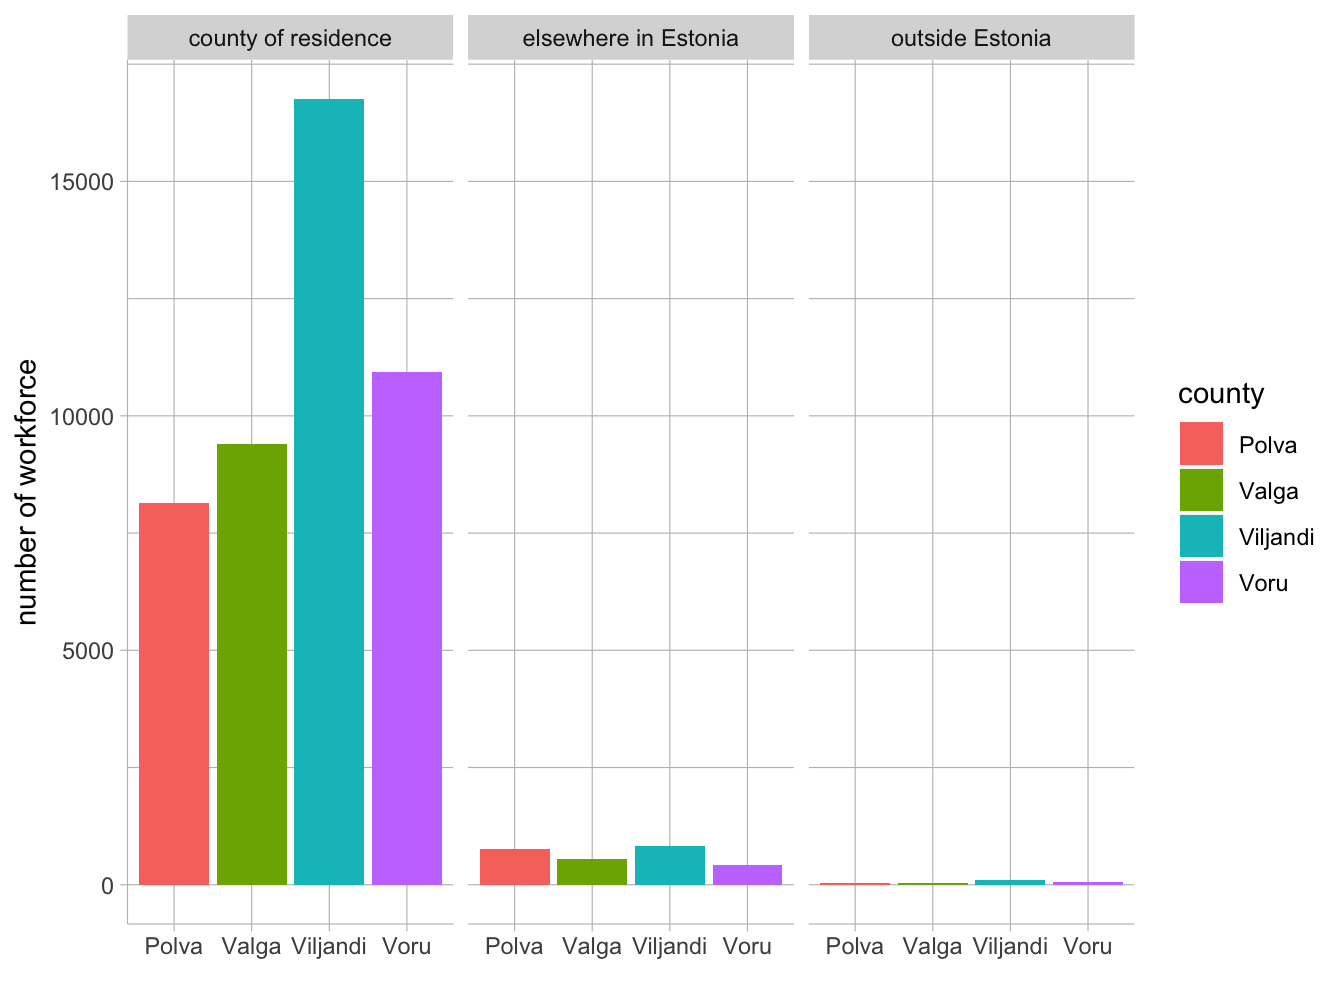
\includegraphics[width=0.8\linewidth]{EIA_2019_digi_files/figure-latex/joonis232-1} 

}

\caption{Viljandi-, Valga-, Võru- ja Põlvamaa elanike töökohtade paiknemine elukoha maakonnas, mujal Eestis või väljaspool Eestit 2000. ja 2011.aastal}\label{fig:joonis232}
\end{figure}

Ehkki põllumajanduses toimusid peamised tööhõive muutused juba 1990.~aastatel, ei ole hõive vähenemine
siiani peatunud. Lõuna-Eesti nelja maakonna koguhõive on püsinud stabiilsena alates 2000.~aastate algusest
(63~000 töötajat 2001. aastal), kuid elukoha lähedal on vähem töökohti, mistõttu on kasvanud tööalane
pendelränne (joonis \ref{fig:joonis232}). Kui 2000. aastal töötas enamik Lõuna-Eesti maakondade töötavast elanikkonnast
oma kodumaakonnas, siis 2011. aastaks töötas 23\% väljaspool maakonda ja 7\% väljaspool Eestit. See
tähendab, et paljud pendelrändajad viibivad kodupiirkonnas ainult nädalavahetustel või veelgi harvem,
mistõttu pikemas perspektiivis võivad ka nende pered sealt lahkuda. Majanduse ümberkorraldumine ning
uued elukorralduslikud ja pendelrände mustrid toetavad rahvastiku vähenemise nõiaringi, viies oluliste
avalike teenuste, sealhulgas koolide kadumiseni, mis omakorda süvendab rahvastiku vähenemist.

\hypertarget{maapiirkondade-ja-vaikelinnade-habimargistamine-suvendab-veelgi-nende-aaremaastumist}{%
\subsection{Maapiirkondade ja väikelinnade häbimärgistamine süvendab veelgi nende ääremaastumist}\label{maapiirkondade-ja-vaikelinnade-habimargistamine-suvendab-veelgi-nende-aaremaastumist}}

Inimkapitali kaoga seotud objektiivsete näitajate kõrval on ääremaastumisel ka selgelt subjektiivne mõõde.
Eesti maapiirkondade ja väikelinnade sotsialismijärgse rahvastikukaoga käsikäes halveneb maapiirkondade
kuvand, mis talupoegliku taustaga identiteedi tõttu on Eestis ajalooliselt olnud väga positiivne. Koos
piirkondliku ebavõrdsuse süvenemise, põllumajandussektori kahanemise ja linnapiirkondade kiire kasvuga
muutub ka maaelu tähendus. Praegu seostuvad maapiirkonnad ja väikelinnad vähem põllumajanduse ning
enam puhkemajanduse ja turismiga (Raagmaa ja Noorkõiv 2013). Kuigi see suundumus toetab turistide ja
maakodu ostjate ligimeelitamiseks idüllilise maaelu ja looduse kuvandi loomist, peegeldavad
maapiirkondade ja väikelinnade sotsialismijärgset rahvastikukadu üha negatiivsemad kirjeldused, mis
samastavad maapiirkondi ääremaaga.

Negatiivsel kuvandil on potentsiaal ääremaid häbimärgistada, mõjutades inimeste otsust neid paiku
külastada, sinna investeerida või elama asuda, seeläbi ühtlasi süvendades ka objektiivset ääremaastumist
(Plüschke-Altof 2017). Seepärast on oluline mõista, kuidas tekivad kohakuvandid. Alates poliitikast ja
turundusest kuni teadus- ja populaarkirjanduseni on avaliku arutelu laiema publikuni viimise eri platvormide
seas väga oluline roll meediakanalitel. Demokraatlikus süsteemis on väga oluline küsimus, kes saab sõna ja
keda kuulatakse. Ehkki ajakirjandusvabadus tagab kõigile ühiskonnaliikmetele võimaluse oma seisukohti
väljendada ja Eesti on selle poolest rahvusvaheliselt kõrgelt hinnatud, näitab mõjukate Eesti ajalehtede ning
arvamusliidrite ja ajalehetoimetajatega tehtud intervjuude diskursuseanalüüs (Plüschke-Altof 2017), et
ääremaade kuvandit toodab arvamuseliit. See koosneb peamiselt ajakirjanikest, teadlastest, poliitikutest
ning kultuuri- ja kunstiinimestest, kes esindavad linlikke institutsioone nagu meediaväljaanded, riigiasutused, ülikoolid või kultuuriasutused (umbes 86\% autoritest, joonis \ref{fig:joonis233}). Ajalehtede suure lugejaskonna tõttu mõjutab eliidi arutelu{[}s regionaalarengu ja ääremaastumise üle esitatav maapiirkondade kuvand{]} ka otsustajaid ning maapiirkondade ja väikelinnade elanikke, kes aga ise on arutellu vähem kaasatud.

\begin{figure}

{\centering 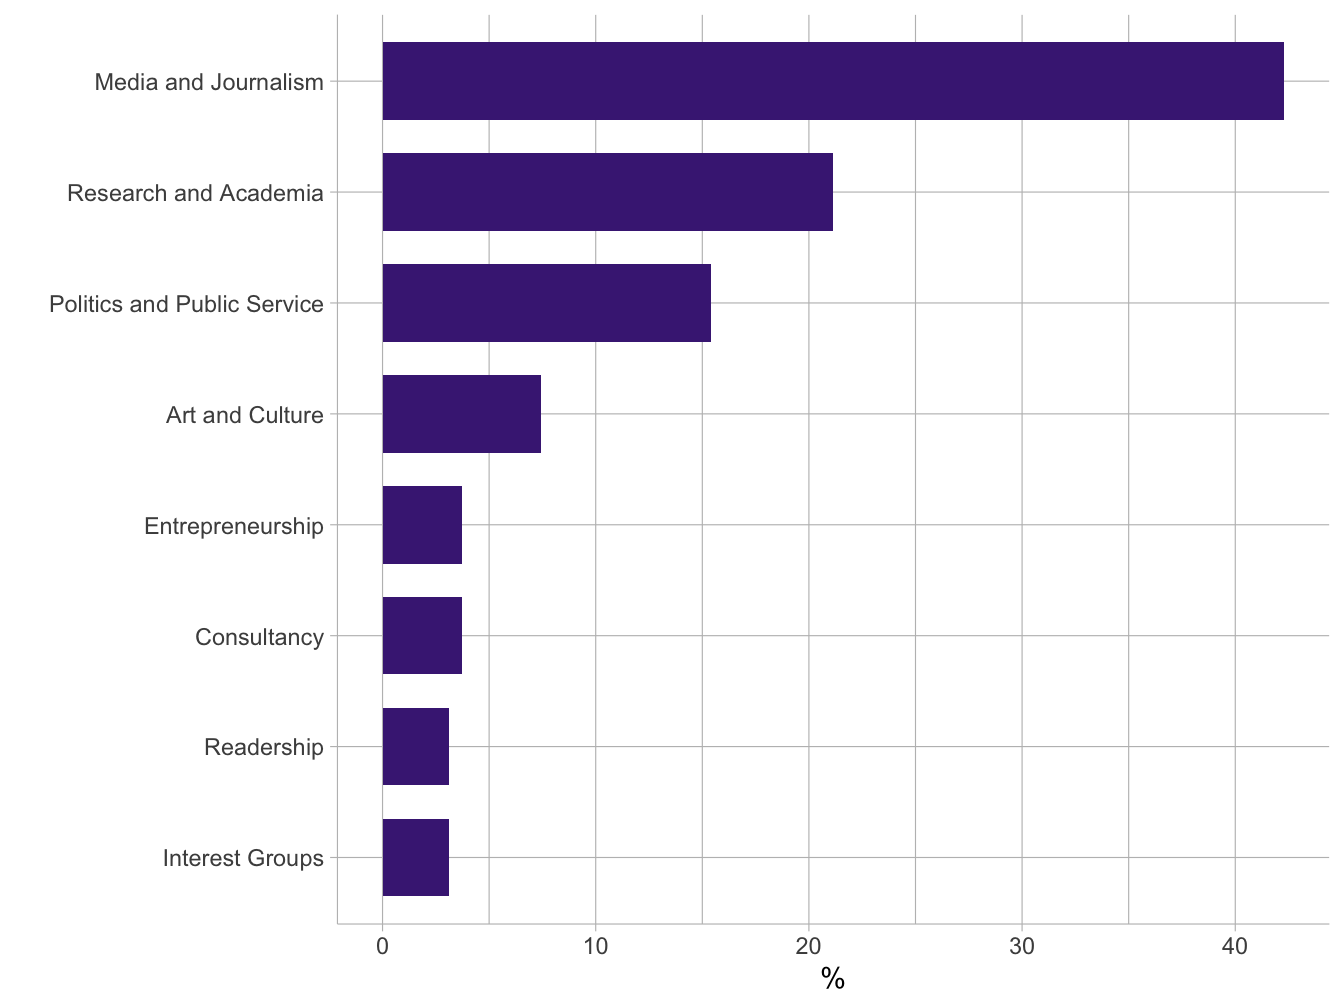
\includegraphics[width=0.8\linewidth]{EIA_2019_digi_files/figure-latex/joonis233-1} 

}

\caption{Kes kujundavad maapiirkondade kuvandit Eesti trükimeedias?}\label{fig:joonis233}
\end{figure}

Meedias seostatakse ääremaad enamasti maapiirkondadega (52\% juhtudest), viidates konkreetsetele
maakohtadele või maapiirkondadele üldiselt, jättes konkreetsed kohad nimetamata (vt joonis \ref{fig:joonis234}).
Piirkondade polariseerumist peegeldab asjaolu, et paljudes artiklites kirjeldatakse ääremaana kogu Eestit
väljaspool Tallinnat ja selle ümbrust. Harvem käsitletakse ääremaad globaalses või ELi kontekstis (42\%) ja
veel palju vähem kõneldakse linnalisest ääremaast (3\%). Maapiirkondade samastamine ääremaaga võib olla
nende jaoks häbimärk, sest ääremaad ei kirjeldata neutraalselt, vaid majanduslikult mahajäänu,
geograafiliselt kauge, poliitiliselt sõltuva, institutsiooniliselt hõreda ja sotsiaalselt probleemsena. Mõnel juhul võimendab maapiirkondade -- või õieti mittelinnaliste piirkondade -- ääremaakuvandit ka narratiiv, mis
rõhutab ääremaa kogukondade vastutust kohaliku arengu (ja ühtlasi mahajäämuse) eest või kujutab neid
omal süül läbikukkumise näidetena. Ajalehtede arvamusartiklites viidatakse näiteks kohalikule
„kolhoosimentaliteedile`` või irratsionaalsele vastuseisule „tänapäevase`` arengu suhtes. Seega maapiirkondi
mitte ainult seostatakse ääremaisusega, vaid pannakse neile ka vastutus, jättes mulje, et maal pole midagi
head, nagu ütleb üks arvamusliider. Kordamise kaudu muutub seos lugejaskonna ja laiema üldsuse silmis
iseenesestmõistetavaks.

\begin{figure}

{\centering 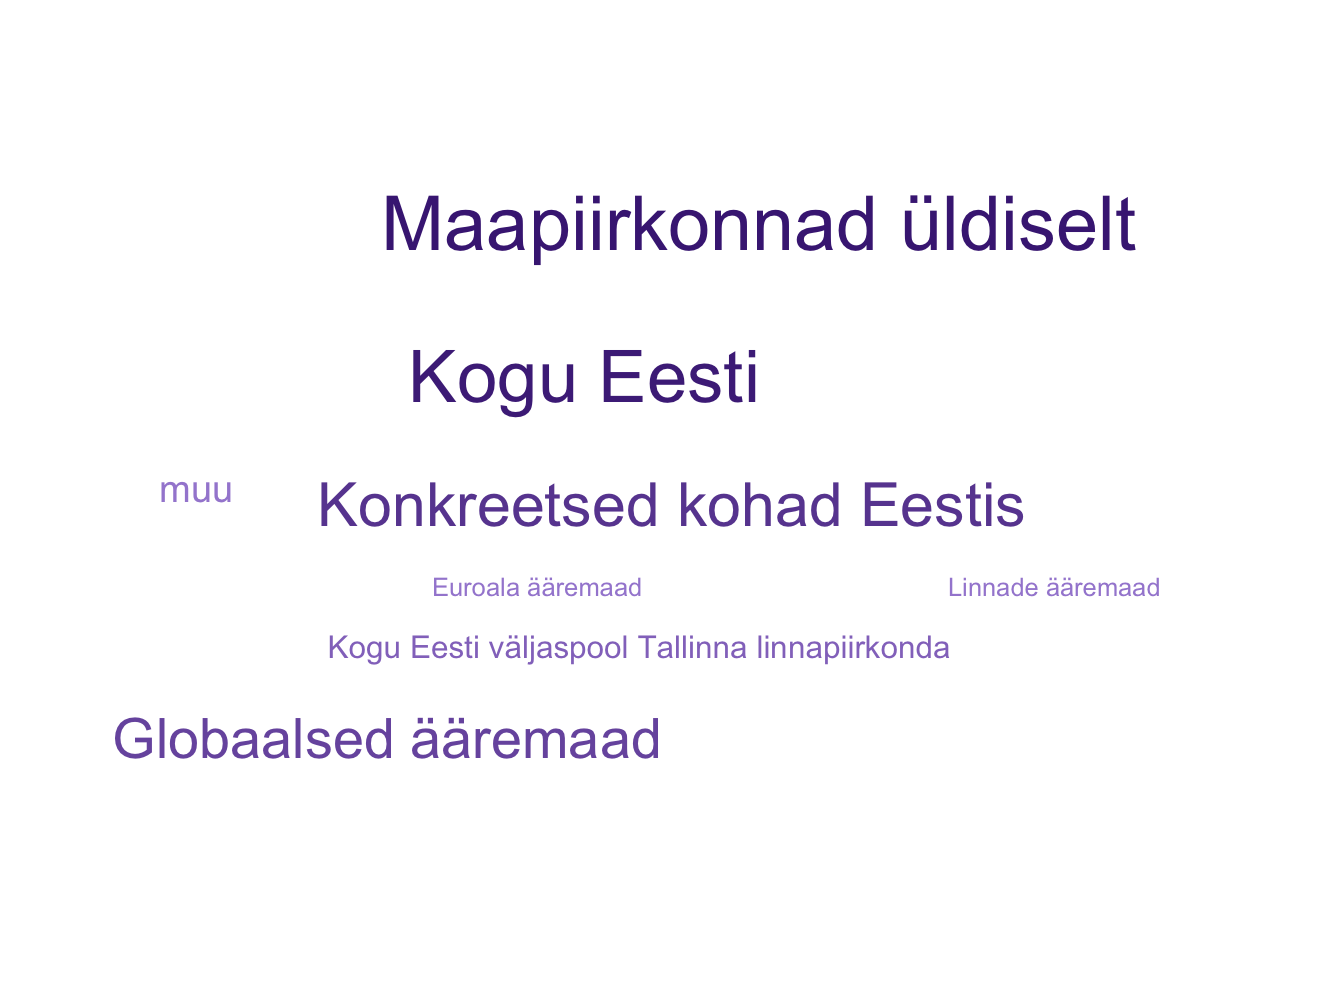
\includegraphics[width=0.8\linewidth]{EIA_2019_digi_files/figure-latex/joonis234-1} 

}

\caption{Mis kohti kirjeldatakse Eesti trükimeedias kui ääremaad?}\label{fig:joonis234}
\end{figure}

Olgugi et meedias domineerib maapiirkondade negatiivne ääremaakuvand, on olemas ka vastudiskursus, mis
toetub olemasolevatele maaelu positiivsetele tähendustele. Siia kuuluvad arvamusartiklid, mis kirjeldavad
maapiirkondi Eesti rahva hällina ühes pärandkultuuri ja puhta loodusega või keskenduvad maaelu
arengueeldustele, näiteks turismi või mahepõllumajandusliku toidutootmise vallas. Lisaks esitavad
arvamusliidrid omasüülise läbikukkumise kuvandile vastukaaluks aktiivse toimetuleku parimaid näiteid. Teine
strateegia on rõhutada kohaliku vastutuse piire, mille seavad mitmel tasandil (nt maailmamajanduses,
riigihalduses, regionaalpoliitikas) toimivad sõltuvussuhted ja ääremaade eiramine Eesti neoliberaalse
regionaalpoliitika tulemusena. Idüllilise maaelu ja kohaliku sõltumuse narratiividega püütakse veenda
lugejaid, et riik peaks regionaalarengusse sekkuma. Nii kujutataks maapiirkondade ja väikelinnade saatust
kui „Eesti rahva elu ja surma küsimus'', nagu ütleb üks teine arvamusliider. See vastudiskursus aga on
maapiirkondade kui omasüülise ääremaa häbimärgistamisega võrreldes siiski alaesindatud.

Maapiirkondade, väikelinnade ja tööstusjärgsete piirkondade ääremaastumine, nagu oleme seda siiani
kirjeldanud, on kestnud juba kolmkümmend aastat. Maapiirkondade rahvastiku, töökohtade (eeskätt
primaarsektoris) ja teenuste vähenemine on käivitanud ääremaastumise tsükli, mida käivitab üleilmne
linnastumine ja nõukogudejärgne majanduse ümberkorraldumine. Need objektiivsed protsessid on läbi
põimunud maapiirkondade muutuva kuvandi ja häbimärgistamisega, mille tulemusel maapiirkonda kui sellist
samastatakse üha enam ääremaaga. Järgnev Eesti regionaalpoliitika ja kohaliku tasandi
ääremaastumisvastaste strateegiate analüüs näitab, et neid omavahel põimunud protsesse on võimendanud
kohaneutraalne, Euroopa piirkondliku konkurentsivõime trende järgiv regionaalpoliitika, mis ei ole
piirkondlikku ebavõrdsust vähendanud.

\hypertarget{konkurentsivoimel-pohinev-regionaalpoliitika-ei-ole-piirkondade-polariseerumist-vahendanud}{%
\subsection{Konkurentsivõimel põhinev regionaalpoliitika ei ole piirkondade polariseerumist vähendanud}\label{konkurentsivoimel-pohinev-regionaalpoliitika-ei-ole-piirkondade-polariseerumist-vahendanud}}

ELi ühtekuuluvuspoliitikas nihkus 2000. aastatel rõhk heaolu jaotavalt lähenemisviisilt konkurentsivõimel ja
innovatsioonil põhinevale poliitikale ning samal ajal ehitati uutes liikmesriikides üles institutsioone ja
kujundati poliitikat. Kuigi piirkondliku toetuse peamised põhimõtted pandi paika juba 1990. aastatel, ei olnud
nende rakendamiseks piisavalt raha. Seepärast olid 2000. aastatel suured ootuse seoses ELi vahenditest
riikide ja piirkondade majandusse lisarahastuse saabumisega. Siiski ei ole enneolematult suur välisrahastus
olnud piisav riigisisese piirkondlikku ebavõrdsuse leevendamiseks. Seda enam et kui Eesti 2004. aastal ELi
astus, asuti ühtekuuluvuspoliitika eesmärke rakendama tsentraalselt ja kohaneutraalselt.

\begin{blockquote}
Kaunid kunstid, teadused, professionaalne ja harrastuslik omalooming
moodustavad vaid väikese osa kultuurist selle sõna laiemas,
antropoloogilises tähenduses.
\end{blockquote}

Piirkondi ja nende arengut eristava kohatundliku lähenemise asemel käsitles Euroopa Komisjon Eestit ühtse
tervikuna. See võimaldas ajada riiklikule majanduskasvule suunatud tsentraalset regionaalpoliitikat (Loewen
2018), milles Eesti on võrreldes teiste liikmesriikide ja eriti sotsialismijärgsete riikidega olnud edukas
\autocite{euroopakomisjon2017}. Eduloo taga peitub aga tegelikult märkimisväärne ebavõrdsus riigi eri piirkondade
vahel (Loewen 2018). Sellal kui ühtekuuluvuspoliitika keskendub ka praegusel programmitöö perioodil
piirkondlikule konkurentsivõimele ja innovatsioonile, on poliitika riiklikul tasandil rakendamine sageli
kasulikum linnapiirkondadele, eriti vähem arenenud riikides (Loewen ja Schulz 2019). Seepärast on
ühtekuuluvuspoliitika pärast toimunud nihet vastuolus traditsioonilise ühtekuuluvuse käsitusega ning võib
linnade ja maapiirkondade vahelise lõhe leevendamise asemel seda tegelikult hoopis süvendada.

Pärast Eestis 15 aastat kestnud ühtekuuluvuspoliitika ajamist tuleb küsida, kas kohaneutraalse lähenemisega
tasub jätkata. Seda enam, et iroonilisel kombel võidakse tsentraliseeritud regionaalpoliitika rakendamisel
saavutatud edu tõttu Eestile järgmisel ELi eelarveperioodil (2012--2017) vähem vahendeid eraldada, sest
tõenäoliselt Eesti kaotab senise vähem arenenud riigi staatuse. Kuna välisvahendid on ka edaspidi Eesti
regionaalarengu peamine ressurss, tuleb luua uusi võimalusi piirkondlikku arengusse sekkumiseks,
ühtlustades regionaalpoliitikat ja muud valdkondlikku poliitikat.

\hypertarget{aaremaa-staatus-ja--kuvand-piiravad-koha-konkurentsivoimet}{%
\subsection{Ääremaa-staatus ja -kuvand piiravad koha konkurentsivõimet}\label{aaremaa-staatus-ja--kuvand-piiravad-koha-konkurentsivoimet}}

Ääremaastumise objektiivsete ja subjektiivsete protsesside taustal, mida võimendab konkurentsivõimel ja
innovatsioonil põhinev regionaalpoliitika, on paljud Eesti maapiirkonnad ja väikelinnad asunud otsima
võimalusi kohaliku arengu edendamiseks. Põllumajanduse ja rasketööstuse väheneva osatähtsusega
arvestades on 2000. aastate algusest peale ELi rahastamiskavadest muude strateegiate seas toetatud
maapiirkondade majanduse mitmekesistamist (nt LEADER). See hõlmab üha enam ka mainekujunduse
strateegiaid (nt kohaturundust ja -brändimist). Kohalike arengukavade järgi loeb rõhuv enamik (2018. aasta
seisuga 83\%) Eesti valdasid mainekujundust üheks oma arengustrateegiaks. See hõlmab
mainekujundusürituste korraldamist, omavalitsuse kuvandi jälgimist ja aktiivset kohaturundust. Ka riigi
tasandil leidub maaelu positiivseid külgi esile tõstvaid laiemale avalikkusele suunatud
mainekujundusalgatusi, teiste seas näiteks „Tule maale`` ja „Maale elama`` (Juhtumikast 1).

\BeginKnitrBlock{casebox}
\hypertarget{juhtumikast-1.-maaelu-edendamine-aaremaastumise-vastu-voitlemiseks-maapiirkondade-mainekujunduse-algatused.}{%
\subsubsection*{Juhtumikast 1. Maaelu edendamine ääremaastumise vastu võitlemiseks: maapiirkondade mainekujunduse algatused.}\label{juhtumikast-1.-maaelu-edendamine-aaremaastumise-vastu-voitlemiseks-maapiirkondade-mainekujunduse-algatused.}}
\addcontentsline{toc}{subsubsection}{Juhtumikast 1. Maaelu edendamine ääremaastumise vastu võitlemiseks: maapiirkondade mainekujunduse algatused.}

Mõlemad algatused sündisid 2012. aastal veendumusest, et on aeg hakata süstemaatiliselt mõtlema maapiirkondade kuvandi rollile. Ehkki liikumiste juhid Tiit Niilo (Tule maale) ja Ivika Nõgel (Maale elama) ei teadnud enne tegutsema asumist teineteise sarnastest algatustest, ajendas mõlemat sama mõte: maapiirkondade elu tuleb edendada, et peatada elanikkonna ja teenuste kadu. Algatused tegutsevad kahel suunal: 1) aidatakse maale elama asumisest huvitatuid ning 2) reklaamitakse ja turundatakse maakohti laiemale avalikkusele, näiteks korraldades laatasid.

Allikas: \url{http://www.tulemaale.ee/} ja \url{http://maale-elama.ee/}.
\EndKnitrBlock{casebox}

Kuid katseid parandada piirkondade konkurentsivõimet mainekujunduse abil pärsib seesama ääremaa-
staatus ja -kuvand, millest maapiirkonnad püüavad vabaneda, nagu viitavad näiteks Kihnu saarel, Järvamaal,
Mulgimaal ja Setomaal tehtud uuringud (\textcite{grootens2018}; Plüschke-Altof 2017). Kohalike otsustajate ja
elanikega läbi viidud 66 põhjaliku intervjuu alusel selgitati välja kolm peamist mainekujunduse meetodit,
mida kasutatakse Eesti ääremaadel: 1) kuvandi ümberpööramine, 2) enese (strateegiline) ääremaastamine ja
3) nähtavuse püüdlemine. Need ei ole alati teadlikud strateegiad, sest kuvandeid loovad meedia,
turundusettevõtted ja poliitikakujundajad ning need tekivad ka tavadiskursuses. Sellegipoolest mõjutavad
nimetatud strateegiad piirkonna tajumist kohalike elanike seas ja mujal ning seeläbi ka otsuste tegemist.

Kuvandi ümberpööramisel kasutatakse ääremaisust „trumpkaardina`` \autocite{grootens2018}. Nii väidavad
kohalikud otsustajad näiteks Kihnus ja Setomaal, et just ääremaa staatus on võimaldanud neil maaelu idülli
ja kultuurilist pärandit säilitada. Tavapärane linna-maa hierarhia pööratakse pea peale, rõhutades maaelu
positiivseid ja linnaelu negatiivseid külgi, nagu seda tegi näiteks intervjueeritud Setomaa elanik, kelle arvates linnaelu iseloomustab „kuritegevus, narkomaania, liiklus ja {[}muu{]} selline jama''. Kuvandi ümberpööramise pooldajad on tihti väga teadlikud kohakuvandi tähtsusest. Näiteks Mulgimaal intervjueeritud otsustaja märkis, et „asi ei ole niivõrd geograafilises asukohas, kuivõrd selles, kus me inimeste mõtlemises paikneme``. Enese strateegilise ääremaastamise puhul ei püüta ääremaakuvandit ümber pöörata, vaid kasutatakse seda ära, rõhutades kohalike võimaluste piiratust üleüldise ääremaastumisega võitlemisel, ja taotletakse toetust. Küsitakse kriitiliselt, kuidas peaksid omavalitsused parandama piirkondade konkurentsivõimet väga piiratud kohalike ressurssidega, mis Mulgimaal intervjueeritud kohaliku elanikud sõnul tegelikult tähendab „elamist peost suhu``. Kui aga ääremaaks olemist kogetakse nagu oldaks nähtamatu või „valge laik kaardil`` \autocite{grootens2018}, näiteks Järvamaal, on peamine eesmärk „olla suurel pildil, suures plaanis`` (ibid.).

Samas aga pärsib ääremaastumine maapiirkondade võimalust mainekujunduse abil konkurentsivõimet
suurendada. Kuigi kuvandi ümberpööramine ja nähtavuse püüdlemine on kooskõlas konkurentsivõimet
taotleva kohaturunduse ideega, nõuab nende edukas rakendamine kultuurilisi, poliitilisi, majanduslikke ja
inimressursse, mis perifeersetes piirkondades sageli puuduvad. Seega seavad piiranguid koha ääremaa-
staatusest tulenevad objektiivsed tegurid nagu rahapuudus, vähene inimkapital või ajakirjanduslike ja
poliitiliste sidemete puudumine. Peale selle on omavalitsustel oht püsivaid kohalikke probleeme pisendada
ja neist üle libiseda või luua õõnes kuvand, mis ei põhine kohalikul olukorral; samuti võib juhtuda, et nad
reklaamivad kõiki maapiirkondi iseloomustavaid üldisi omadusi (Plüschke-Altof 2017; Grootens 2018). Nii ei
jää paljudel maapiirkondadel ja väikelinnadel muud üle, kui valida enese ääremaastamise strateegia. Ehkki
see lähenemine kuvandikasutusele pakub võimalust avatult tegeleda kohalike probleemidega ning nõuda toetust ja rohkem ümberjaotamisele suunatud regionaalpoliitikat, muutub see ääremaa-kuvandi häbimärgistava toime (subjektiivsete tegurite) tõttu koormaks kohalikule arengule. Mainekujundus illustreerib seega konkurentsivõimel põhineva regionaalpoliitika paradokse piirkondliku ebavõrdsuse
kontekstis, kus kohaliku arengu jaoks vajalikud ressursid on ebaühtlaselt jaotatud, ning nõuab ulatuslikumal
ümberjaotamisel põhinevat poliitikat.

\hypertarget{regionaalpoliitika-edendamine-objektiivse-ja-subjektiivse-aaremaastumisega-voitlemise-teel}{%
\subsection{Regionaalpoliitika edendamine objektiivse ja subjektiivse ääremaastumisega võitlemise teel}\label{regionaalpoliitika-edendamine-objektiivse-ja-subjektiivse-aaremaastumisega-voitlemise-teel}}

Selgitasime, et Eestis on ääremaastumine mitmemõõtmeline ja -tasandiline protsess, mis mõjutab eriti maapiirkondi, aga ka riiki tervikuna. See hõlmab objektiivseid protsesse, sealhulgas valikulist väljarännet, majanduslangust ja osutatavate teenuste vähenemist. Lisaks aga mõjutab see ka maapiirkondade subjektiivset kuvandit, põhjustades regionaalse polariseerumise tõttu maapiirkondade vähest nähtavust ja territoriaalset häbimärgistamist. Selle vastu võitlemisel on Eesti regionaalpoliitikas järgitud neoliberaalseid suundumusi, püüdes kohalikku arengut edendada piirkondade konkurentsivõime ja innovatsiooni toetamise teel. Kuid riigi tasandil rakendatuna võib seesugune kohaneutraalne mittesekkumispoliitika maaelu arengut hoopis takistada, eelistades lõppkokkuvõttes linnapiirkondi. Kuna peagi tõenäoliselt muutub Eesti staatus ELi ühtekuuluvuspoliitikas, avaneb võimalus arutada, kuidas arenguressursid võiksid jõuda ääremaadele. Seda arutelu soosides on lootust katkestada nõiaring, mis taastoodab suurte linnapiirkondade ja ülejäänud riigi omavahelist polariseerumist.

\hypertarget{viidatud-allikad-1}{%
\subsection*{Viidatud allikad}\label{viidatud-allikad-1}}
\addcontentsline{toc}{subsection}{Viidatud allikad}

\printbibliography[segment=\therefsegment,heading=subbibliography]

\hypertarget{chapter24}{%
\section{Autostumine ja ligipääsetatuvuse muutused Eestis}\label{chapter24}}

\hypertarget{chapter30}{%
\chapter{Loodusruum}\label{chapter30}}

\hypertarget{sissejuhatus-2}{%
\subsection*{Sissejuhatus}\label{sissejuhatus-2}}
\addcontentsline{toc}{subsection}{Sissejuhatus}

Lorem ipsum dolor sit amet, consectetur adipiscing elit, sed do eiusmod tempor incididunt ut labore et dolore magna aliqua. Ultrices sagittis orci a scelerisque purus. Auctor urna nunc id cursus metus aliquam. Malesuada fames ac turpis egestas sed tempus urna et pharetra. Non diam phasellus vestibulum lorem. Fermentum iaculis eu non diam phasellus vestibulum. Imperdiet nulla malesuada pellentesque elit eget gravida cum sociis natoque. Elit pellentesque habitant morbi tristique senectus. Pulvinar neque laoreet suspendisse interdum consectetur. Sit amet nisl purus in mollis. Dignissim suspendisse in est ante in. Pretium viverra suspendisse potenti nullam ac tortor. Tellus cras adipiscing enim eu turpis egestas pretium. Sit amet volutpat consequat mauris nunc. Euismod quis viverra nibh cras pulvinar mattis nunc sed blandit. Iaculis nunc sed augue lacus viverra vitae congue eu consequat.

Facilisis mauris sit amet massa. Nisi porta lorem mollis aliquam ut porttitor leo. Aliquet nibh praesent tristique magna sit amet. Orci nulla pellentesque dignissim enim sit amet. Egestas sed sed risus pretium quam. Elementum integer enim neque volutpat ac tincidunt vitae semper quis. Sit amet mattis vulputate enim. Urna et pharetra pharetra massa massa ultricies mi quis hendrerit. Enim facilisis gravida neque convallis a cras semper. Scelerisque eu ultrices vitae auctor eu augue.

Neque ornare aenean euismod elementum nisi. Id faucibus nisl tincidunt eget nullam non nisi. Convallis convallis tellus id interdum velit laoreet id donec ultrices. Ac feugiat sed lectus vestibulum mattis ullamcorper. Ultrices eros in cursus turpis massa. Mi sit amet mauris commodo quis imperdiet massa tincidunt nunc. In nulla posuere sollicitudin aliquam ultrices sagittis orci a scelerisque. Pellentesque adipiscing commodo elit at imperdiet. Egestas congue quisque egestas diam in arcu. Eget nunc scelerisque viverra mauris in aliquam sem fringilla ut. Pretium aenean pharetra magna ac placerat vestibulum lectus mauris. Sit amet mauris commodo quis imperdiet massa tincidunt nunc pulvinar. Amet porttitor eget dolor morbi non.

\hypertarget{chapter31}{%
\section{Looduskeskkonna kasutamine}\label{chapter31}}

\begin{authors}
\textbf{Tiit, Teet (Eluülikool)}
\end{authors}

\begin{points}
\begin{itemize}
\item
  Lorem ipsum dolor sit amet, consectetur adipiscing elit, sed do
  eiusmod tempor incididunt ut labore et dolore magna aliqua.
\item
  Auctor urna nunc id cursus metus aliquam. Malesuada fames ac turpis
  egestas sed tempus urna et pharetra
\item
  Ultrices sagittis orci a scelerisque purus
\end{itemize}
\end{points}

Lorem ipsum dolor sit amet, consectetur adipiscing elit, sed do eiusmod tempor incididunt ut labore et dolore magna aliqua. Ultrices sagittis orci a scelerisque purus. Auctor urna nunc id cursus metus aliquam. Malesuada fames ac turpis egestas sed tempus urna et pharetra. Non diam phasellus vestibulum lorem. Fermentum iaculis eu non diam phasellus vestibulum. Imperdiet nulla malesuada pellentesque elit eget gravida cum sociis natoque. Elit pellentesque habitant morbi tristique senectus. Pulvinar neque laoreet suspendisse interdum consectetur. Sit amet nisl purus in mollis. Dignissim suspendisse in est ante in. Pretium viverra suspendisse potenti nullam ac tortor. Tellus cras adipiscing enim eu turpis egestas pretium. Sit amet volutpat consequat mauris nunc. Euismod quis viverra nibh cras pulvinar mattis nunc sed blandit. Iaculis nunc sed augue lacus viverra vitae congue eu consequat.

\begin{blockquote}
Lorem ipsum dolor sit amet, consectetur adipiscing elit, sed do eiusmod
tempor incididunt ut labore et dolore magna aliqua. Ultrices sagittis
orci a scelerisque purus.
\end{blockquote}

Sit amet nisl purus in mollis. Dignissim suspendisse in est ante in. Pretium viverra suspendisse potenti nullam ac tortor.

\hypertarget{chapter32}{%
\section{Looduskeskkonna mõju inimestele ja ühiskonnale}\label{chapter32}}

\hypertarget{chapter33}{%
\section{Looduskeskkonna kujundamine avalikuks kasutuseks}\label{chapter33}}

\hypertarget{chapter34}{%
\section{Kaasarääkimise võimalused avaliku ruumi kujundamises}\label{chapter34}}

\hypertarget{chapter40}{%
\chapter{Linna- ja arhitektuurne ruum}\label{chapter40}}

\hypertarget{sissejuhatus-3}{%
\subsection*{Sissejuhatus}\label{sissejuhatus-3}}
\addcontentsline{toc}{subsection}{Sissejuhatus}

Lorem ipsum dolor sit amet, consectetur adipiscing elit, sed do eiusmod tempor incididunt ut labore et dolore magna aliqua. Ultrices sagittis orci a scelerisque purus. Auctor urna nunc id cursus metus aliquam. Malesuada fames ac turpis egestas sed tempus urna et pharetra. Non diam phasellus vestibulum lorem. Fermentum iaculis eu non diam phasellus vestibulum. Imperdiet nulla malesuada pellentesque elit eget gravida cum sociis natoque. Elit pellentesque habitant morbi tristique senectus. Pulvinar neque laoreet suspendisse interdum consectetur. Sit amet nisl purus in mollis. Dignissim suspendisse in est ante in. Pretium viverra suspendisse potenti nullam ac tortor. Tellus cras adipiscing enim eu turpis egestas pretium. Sit amet volutpat consequat mauris nunc. Euismod quis viverra nibh cras pulvinar mattis nunc sed blandit. Iaculis nunc sed augue lacus viverra vitae congue eu consequat.

Facilisis mauris sit amet massa. Nisi porta lorem mollis aliquam ut porttitor leo. Aliquet nibh praesent tristique magna sit amet. Orci nulla pellentesque dignissim enim sit amet. Egestas sed sed risus pretium quam. Elementum integer enim neque volutpat ac tincidunt vitae semper quis. Sit amet mattis vulputate enim. Urna et pharetra pharetra massa massa ultricies mi quis hendrerit. Enim facilisis gravida neque convallis a cras semper. Scelerisque eu ultrices vitae auctor eu augue.

Neque ornare aenean euismod elementum nisi. Id faucibus nisl tincidunt eget nullam non nisi. Convallis convallis tellus id interdum velit laoreet id donec ultrices. Ac feugiat sed lectus vestibulum mattis ullamcorper. Ultrices eros in cursus turpis massa. Mi sit amet mauris commodo quis imperdiet massa tincidunt nunc. In nulla posuere sollicitudin aliquam ultrices sagittis orci a scelerisque. Pellentesque adipiscing commodo elit at imperdiet. Egestas congue quisque egestas diam in arcu. Eget nunc scelerisque viverra mauris in aliquam sem fringilla ut. Pretium aenean pharetra magna ac placerat vestibulum lectus mauris. Sit amet mauris commodo quis imperdiet massa tincidunt nunc pulvinar. Amet porttitor eget dolor morbi non.

\hypertarget{chapter41}{%
\section{Avalik ruum ruumiloomes}\label{chapter41}}

\begin{authors}
\textbf{Tiit, Teet (Eluülikool)}
\end{authors}

\begin{points}
\begin{itemize}
\item
  Lorem ipsum dolor sit amet, consectetur adipiscing elit, sed do
  eiusmod tempor incididunt ut labore et dolore magna aliqua.
\item
  Auctor urna nunc id cursus metus aliquam. Malesuada fames ac turpis
  egestas sed tempus urna et pharetra
\item
  Ultrices sagittis orci a scelerisque purus
\end{itemize}
\end{points}

Lorem ipsum dolor sit amet, consectetur adipiscing elit, sed do eiusmod tempor incididunt ut labore et dolore magna aliqua. Ultrices sagittis orci a scelerisque purus. Auctor urna nunc id cursus metus aliquam. Malesuada fames ac turpis egestas sed tempus urna et pharetra. Non diam phasellus vestibulum lorem. Fermentum iaculis eu non diam phasellus vestibulum. Imperdiet nulla malesuada pellentesque elit eget gravida cum sociis natoque. Elit pellentesque habitant morbi tristique senectus. Pulvinar neque laoreet suspendisse interdum consectetur. Sit amet nisl purus in mollis. Dignissim suspendisse in est ante in. Pretium viverra suspendisse potenti nullam ac tortor. Tellus cras adipiscing enim eu turpis egestas pretium. Sit amet volutpat consequat mauris nunc. Euismod quis viverra nibh cras pulvinar mattis nunc sed blandit. Iaculis nunc sed augue lacus viverra vitae congue eu consequat.

\begin{blockquote}
Lorem ipsum dolor sit amet, consectetur adipiscing elit, sed do eiusmod
tempor incididunt ut labore et dolore magna aliqua. Ultrices sagittis
orci a scelerisque purus.
\end{blockquote}

Sit amet nisl purus in mollis. Dignissim suspendisse in est ante in. Pretium viverra suspendisse potenti nullam ac tortor.

\hypertarget{chapter42}{%
\section{Kultuuripärand ja ruumikvaliteet}\label{chapter42}}

\hypertarget{chapter43}{%
\section{Aktivism ruumiloomes}\label{chapter43}}

\hypertarget{chapter44}{%
\section{Ruumiandmete roll planeerimises}\label{chapter44}}

\hypertarget{chapter50}{%
\chapter{Tulevikustsenaariumid}\label{chapter50}}

Lorem ipsum dolor sit amet, consectetur adipiscing elit, sed do eiusmod tempor incididunt ut labore et dolore magna aliqua. Ultrices sagittis orci a scelerisque purus. Auctor urna nunc id cursus metus aliquam. Malesuada fames ac turpis egestas sed tempus urna et pharetra. Non diam phasellus vestibulum lorem. Fermentum iaculis eu non diam phasellus vestibulum. Imperdiet nulla malesuada pellentesque elit eget gravida cum sociis natoque. Elit pellentesque habitant morbi tristique senectus. Pulvinar neque laoreet suspendisse interdum consectetur. Sit amet nisl purus in mollis. Dignissim suspendisse in est ante in. Pretium viverra suspendisse potenti nullam ac tortor. Tellus cras adipiscing enim eu turpis egestas pretium. Sit amet volutpat consequat mauris nunc. Euismod quis viverra nibh cras pulvinar mattis nunc sed blandit. Iaculis nunc sed augue lacus viverra vitae congue eu consequat.

Facilisis mauris sit amet massa. Nisi porta lorem mollis aliquam ut porttitor leo. Aliquet nibh praesent tristique magna sit amet. Orci nulla pellentesque dignissim enim sit amet. Egestas sed sed risus pretium quam. Elementum integer enim neque volutpat ac tincidunt vitae semper quis. Sit amet mattis vulputate enim. Urna et pharetra pharetra massa massa ultricies mi quis hendrerit. Enim facilisis gravida neque convallis a cras semper. Scelerisque eu ultrices vitae auctor eu augue.

Neque ornare aenean euismod elementum nisi. Id faucibus nisl tincidunt eget nullam non nisi. Convallis convallis tellus id interdum velit laoreet id donec ultrices. Ac feugiat sed lectus vestibulum mattis ullamcorper. Ultrices eros in cursus turpis massa. Mi sit amet mauris commodo quis imperdiet massa tincidunt nunc. In nulla posuere sollicitudin aliquam ultrices sagittis orci a scelerisque. Pellentesque adipiscing commodo elit at imperdiet. Egestas congue quisque egestas diam in arcu. Eget nunc scelerisque viverra mauris in aliquam sem fringilla ut. Pretium aenean pharetra magna ac placerat vestibulum lectus mauris. Sit amet mauris commodo quis imperdiet massa tincidunt nunc pulvinar. Amet porttitor eget dolor morbi non.

\hypertarget{chapter51}{%
\section{Mitu kodu on mu kindlus}\label{chapter51}}

\begin{authors}
\textbf{Tiit, Teet (Eluülikool)}
\end{authors}

\begin{points}
\begin{itemize}
\item
  Lorem ipsum dolor sit amet, consectetur adipiscing elit, sed do
  eiusmod tempor incididunt ut labore et dolore magna aliqua.
\item
  Auctor urna nunc id cursus metus aliquam. Malesuada fames ac turpis
  egestas sed tempus urna et pharetra
\item
  Ultrices sagittis orci a scelerisque purus
\end{itemize}
\end{points}

Lorem ipsum dolor sit amet, consectetur adipiscing elit, sed do eiusmod tempor incididunt ut labore et dolore magna aliqua. Ultrices sagittis orci a scelerisque purus. Auctor urna nunc id cursus metus aliquam. Malesuada fames ac turpis egestas sed tempus urna et pharetra. Non diam phasellus vestibulum lorem. Fermentum iaculis eu non diam phasellus vestibulum. Imperdiet nulla malesuada pellentesque elit eget gravida cum sociis natoque. Elit pellentesque habitant morbi tristique senectus. Pulvinar neque laoreet suspendisse interdum consectetur. Sit amet nisl purus in mollis. Dignissim suspendisse in est ante in. Pretium viverra suspendisse potenti nullam ac tortor. Tellus cras adipiscing enim eu turpis egestas pretium. Sit amet volutpat consequat mauris nunc. Euismod quis viverra nibh cras pulvinar mattis nunc sed blandit. Iaculis nunc sed augue lacus viverra vitae congue eu consequat.

\begin{blockquote}
Lorem ipsum dolor sit amet, consectetur adipiscing elit, sed do eiusmod
tempor incididunt ut labore et dolore magna aliqua. Ultrices sagittis
orci a scelerisque purus.
\end{blockquote}

Sit amet nisl purus in mollis. Dignissim suspendisse in est ante in. Pretium viverra suspendisse potenti nullam ac tortor.

\printbibliography


\end{document}
